\documentclass{article}
\usepackage[utf8]{inputenc}
\usepackage{tikz}
\usetikzlibrary{calc}
\usepackage{intcalc}
\usepackage[]{skak}
\usepackage{geometry, colortbl, color}
\geometry{a4paper, top=0.cm, left=1cm, right=1cm, bottom=0cm, includehead, includefoot}

% this makes a table
\newcommand{\pgntable}{
    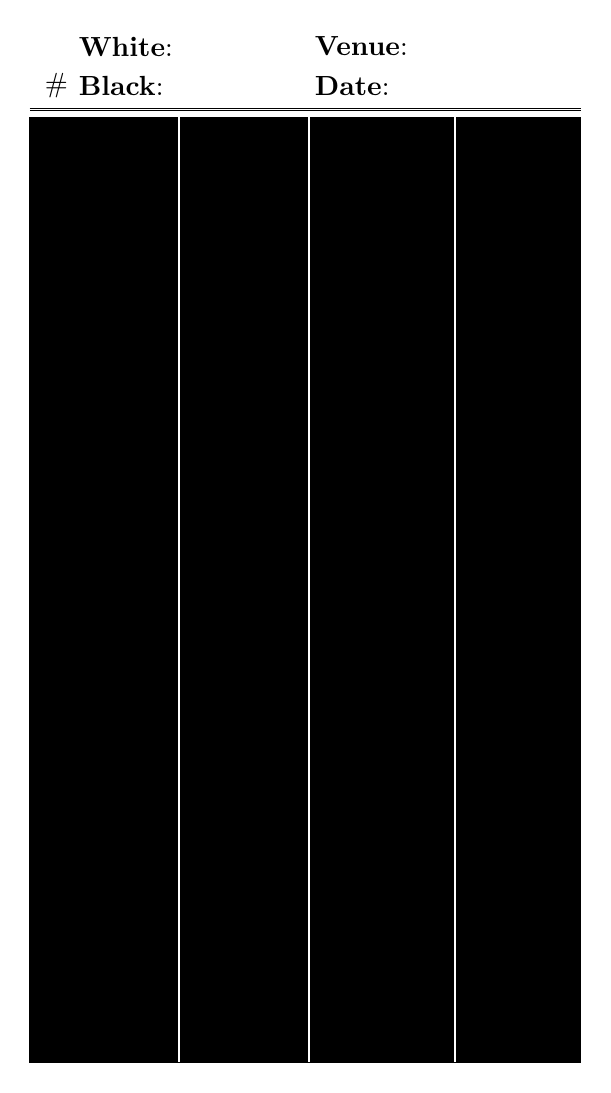
\begin{tikzpicture}
        \def\rowheight{0.4}
        \node[right] at (0.07,0) {\#};
        \node[right] at (0.5,0.5) {\textbf{White}:};
        \node[right] at (0.5, 0) {\textbf{Black}:};
        \node[right] at (3.5,0.5) {\textbf{Venue}:};
        \node[right] at (3.5, 0) {\textbf{Date}:};
        \draw[double] (0,-\rowheight*0.75) -- (7,-\rowheight*0.75);
        \foreach \row in {1,...,30}
        {
            \ifthenelse{\intcalcMod{\row}{2}=1}{\def\clr{white}}{\def\clr{black!10}};
            \draw[fill=\clr, draw=\clr] (0,-\row*\rowheight) rectangle (3.5,-\row*\rowheight-\rowheight);
            \node at (0.3,-\row*\rowheight-\rowheight/2) {\row};
            \draw[fill=\clr, draw=\clr] (3.5,-\row*\rowheight) rectangle (7,-\row*\rowheight-\rowheight);
            \node at (3.8,-\row*\rowheight-\rowheight/2) {\intcalcAdd{30}{\row}};
        }
        \draw[white, thick] (1.9,-\rowheight*0.75-0.1) -- (1.9,-30*\rowheight-\rowheight);
        \draw[white, thick] (3.55,-\rowheight*0.75-0.1) -- (3.55,-30*\rowheight-\rowheight);
        \draw[white, thick] (5.4,-\rowheight*0.75-0.1) -- (5.4,-30*\rowheight-\rowheight);
    \end{tikzpicture}
}

% this fills a page with tables
\newcommand{\pgnpage}{
    \begin{minipage}{0.5\textwidth}
        \pgntable
    \end{minipage}
    ~
    \begin{minipage}{0.5\textwidth}
        \pgntable
    \end{minipage}
    \vfill
    \begin{minipage}{0.5\textwidth}
        \pgntable
    \end{minipage}
    ~
    \begin{minipage}{0.5\textwidth}
        \pgntable
    \end{minipage}
    \newpage
}

\begin{document}
\pagestyle{empty}
%first page
% how to set a board
% \begin{minipage}{0.5\textwidth}
%     \newgame 
%     \showboard
% \end{minipage}
% ~
% % legend
% \begin{minipage}{0.5\textwidth}
% \pgntable
% \end{minipage}
% \vfill
% \begin{minipage}{0.5\textwidth}
% \begin{tabular}{cccc}
% & & Sym & Pts \\
% \hline
% \hline\\[-2ex]
% \symking & King & K & $\infty$ \\
% \symqueen & Queen & Q & 9 \\
% \symrook & Rook & R & 5 \\
% \symbishop & Bishop & B & 3 \\
% \symknight & Knight & N & 3 \\
% \sympawn & Pawn & & 1 \\
% \hline\\[-2ex]
% & Capture & $\times$ & \\
% & King-side castling & 0-0 & \\
% & Queen-sid & 0-0-0 & \\
% & Check & $+$ & \\
% & Checkmate & \# & \\
% \hline\\[-2ex]
% & Good & ! & \\
% & Surprisingly good & !! & \\
% & Bad & ? & \\
% & Blunder & ?? & \\
% \end{tabular}
% \end{minipage}
% ~
% \begin{minipage}{0.5\textwidth}
% \pgntable
% \end{minipage}

% % 3 more pages filled with tables
% \pgnpage
\pgnpage
\pgnpage

\end{document}
